\section{Day 20: Homotopy Constructions (Nov. 14, 2024)}
Outfit of the day: more plaid!!
\begin{figure}[h]
    \centering
    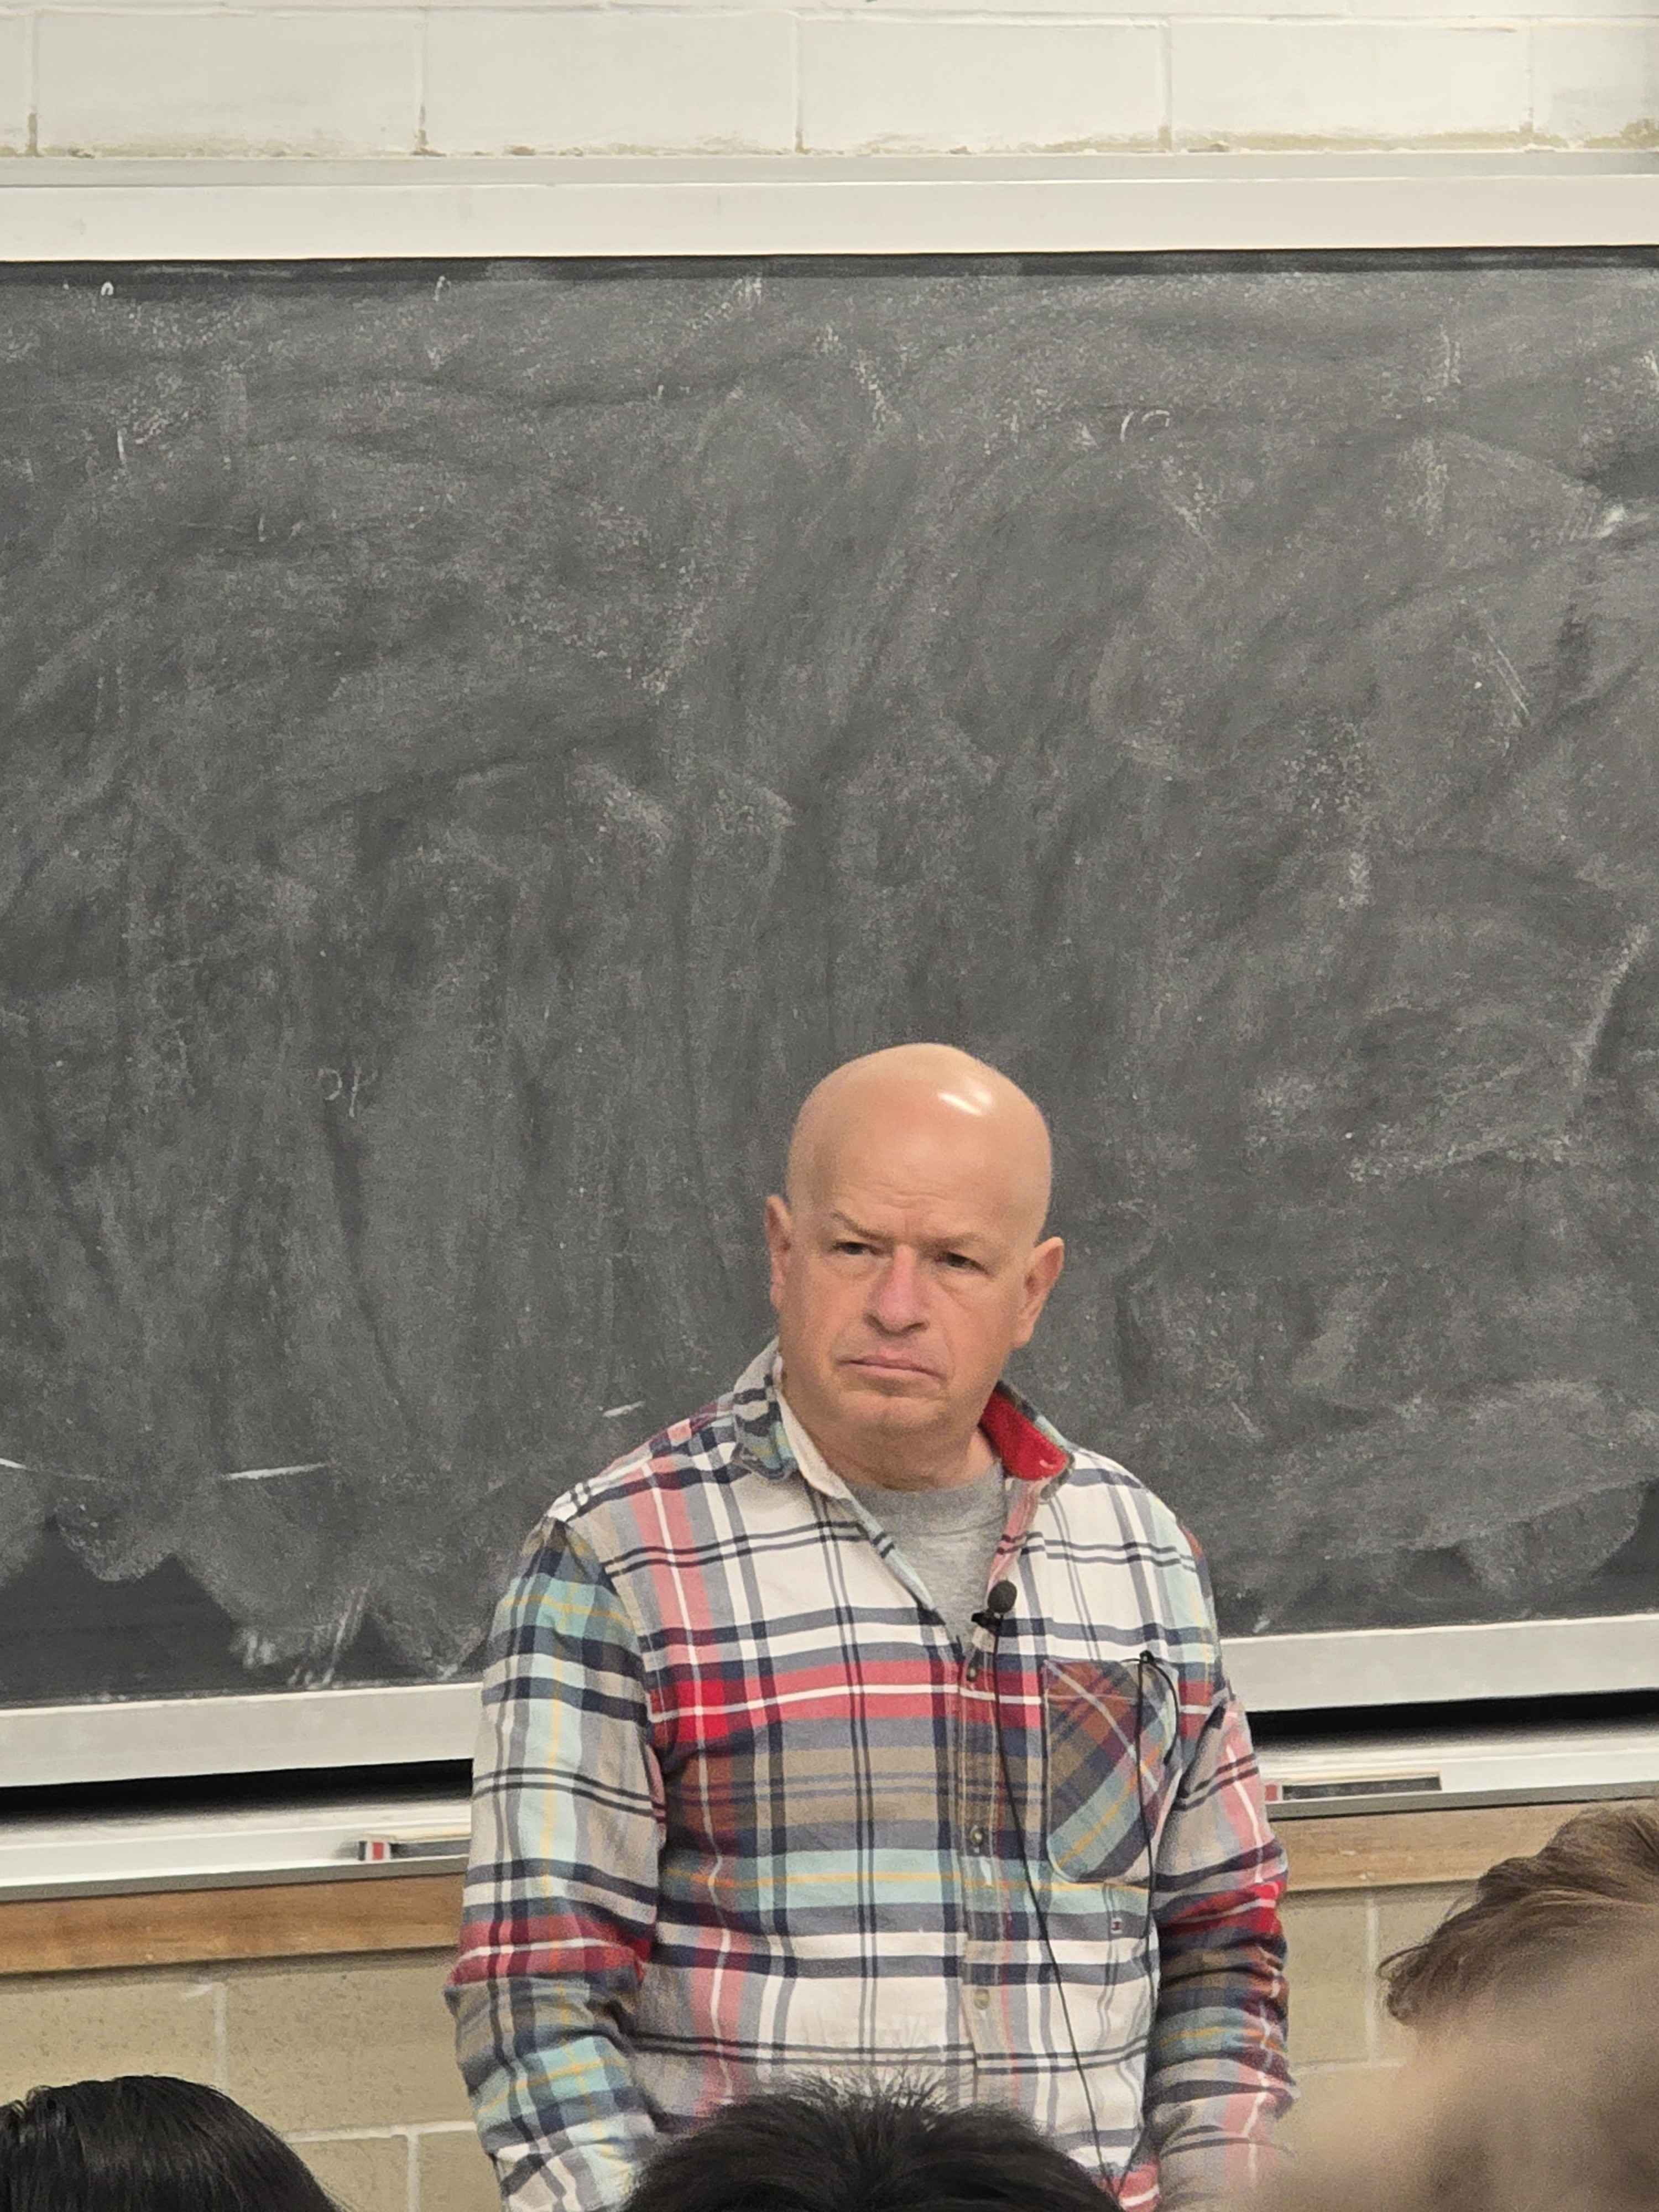
\includegraphics[scale=0.1]{MAT327 Notes/Dror Shirts/dror day 20 shirt.jpg}
\end{figure}

\noindent Recall that we have $[\gamma_1] \ast [\gamma_2] = [\gamma_1 \ast \gamma_2]$ assuming $\gamma_1(1) = \gamma_2(0)$; the operation $\ast$ is a composition of paths, i.e. concatenation (read: product of paths in Munkres). As shown last time, $\ast$ is associative, has identities $[e_x]$, and has inverses $[\gamma] \mapsto [\overline{\gamma}]$. 
\medskip\newline
Let $X$ be a space, and let $x_0$ be a point in $X$. A path in $X$ that begins and ends at $x_0$ is called a loop based at $x_0$, and the set of path homotopy classes of loops based at $x_0$, equipped with $\ast$, is called the fundamental group of $X$ relative to base point $x_0$, denoted by $\pi_1(X, x_0)$.
\medskip\newline
A base space is defined as $(X, x_0)$, where $x_0 \in X$ is called the base point as per above. The convention is that we write $f : (X, x_0) \to (Y, y_0)$ meaning $f : X \to Y$ and $f(x_0) = y_0$, where $f$ is continuous.
\begin{definition}
    Given $(X, x_0)$, $\pi_1(X, x_0) = \{ [\gamma] \mid \gamma : [0, 1] \to X; \gamma(0) = \gamma(1) = x_0 \}$. We see that $\pi_1(X, x_0)$ indeed satisfy the axioms for a group; we write $e = e_{x_0}$, $e_{x_0}(s) = x_0$ for identity.
\end{definition}
\noindent We now give a few examples.
\begin{enumerate}[label=(\alph*)]
    \item $\pi_1(\RR^n, 0) = \{[e_0]\} = \{e\}$ is the trivial group, since if $f$ is a loop in $\RR^n$ based at $0$, the straight-line homotopy is a path homotopy that sends $f$ to the constant path at $0$. Notice that this argument works to show that $\pi_1(X, x_0)$ where $X$ is a convex subset of $\RR^n$ and $x_0 \in X$ is also a trivial group, as these all consist of nothing but $\{[x_0]\}$.
\end{enumerate}
\begin{simplethm}
    If $X$ is path connected and $x_{0, 1} \in X$ then $\pi_1(X, x_0) \cong \pi_1(X, x_1)$, meaning there exists $\varphi : \pi_1(X, x_0) \to \pi_1(X, x_1)$ and $\psi : \pi_1(X, x_1) \to \pi_1(X, x_0)$, where $\varphi, \psi$ are group homomorphisms and inverses of each other. In particular, we say that these are \textit{isomorphisms}.
\end{simplethm}
\noindent Pick a path $\lambda$ such that $\lambda(0) = x_0$, $\lambda(1) = x_1$, and $\lambda(i) = x_i$. Define $\psi : \pi_1(X, x_1) \to \pi_1(X, x_0)$ by $[\gamma] \mapsto [\lambda] \ast [\gamma] \ast [\overline{\lambda}] = [\lambda \ast \gamma \ast \overline{\lambda}]$, where $[\gamma]$ is an element of $\pi_1(X, x_1)$, where we recall that it is the equivalence class of loops $\gamma(0) = \gamma(1) = x_1$. Indeed, this is a group homomorphism. (note that for ease of reading, we omit $\ast$ and just concatenate per convention) We do this by checking that $\psi([\gamma_1][\gamma_2]) = [\lambda \gamma_1 \gamma_2 \overline{\lambda}]$ is equivalent to $\psi([\gamma_1]) \psi([\gamma_2])$, which we may see from the following,
\begin{align*}
    \psi([\gamma_1]) \psi([\gamma_2]) &= [\lambda \gamma_1 \overline{\lambda}] [\lambda \gamma_2 \overline{\lambda}] \\
    &= [\lambda \gamma_1 \overline{\lambda} \lambda \gamma_2 \overline{\lambda}] \\
    &= [\lambda \gamma_1] [\overline{\lambda} \lambda]  [\gamma_2 \overline{\lambda}] \\
    &= [\lambda \gamma_1] [e_{x_1}] [\gamma_2 \overline{\lambda}] \\
    &= [\lambda \gamma_1] [\gamma_2 \overline{\lambda}] \\
    &= [\lambda \gamma_1 \gamma_2 \overline{\lambda}],
\end{align*}
which is the left hand side as desired. We may also check that $\varphi : [\gamma] \mapsto [\overline{\lambda} \gamma \lambda]$ is also a group homomorphism.
\begin{simpleclaim}
    $(\psi \circ \varphi)([\gamma]) = \psi(\overline{\lambda} \gamma \lambda) = [\lambda \overline{\lambda} \gamma \lambda \overline{\lambda}] = [\gamma]$. Thus, $\psi \circ \varphi = \id_{\pi_1(X, x_0)}$.
\end{simpleclaim}
\noindent Obviously, this holds in the other direction as well. \qed

\begin{definition}
    We say that $X$ is \textit{simply connected} if it is path connected and $\pi_1(X, x_0) = \{e\}$ for some $x_0$, i.e. $\pi_1(X, x_0)$ is the trivial (one element) group.
\end{definition}
\noindent Notice that the definition may be modified to say that \textit{all} $\pi_1(X, x_0)$ for all $x_0 \in X$ are trivial, by our previous isomorphism construction. In particular, $\RR^n$ is a simply connected space.
\begin{simplethm}
    Recall that $S^1 = \{x \in \RR^2 \mid \abs{x} = 1\} = \{z \in \CC, \abs{z} = 1\}$. We have that $\pi_1(S^1, 1) \cong \ZZ$. 
\end{simplethm}
\noindent The intuition is that $\pi_1(S^1, 1)$ consists of equivalence classes of paths that stay at $1$, go around the circle once, go around the circle twice, etc... we may then map the number of times that they go around the circle to the integers as desired, with the sign being related to whether the path is clockwise or counterclockwise. However, this is not a proper proof.
\medskip\newline
\noindent Quick digression; in the following diagram,
% https://q.uiver.app/#q=WzAsMyxbMCwyLCJaIl0sWzIsMiwiWSJdLFsyLDAsIlgiXSxbMCwyLCJcXHRpbGRle2Z9Il0sWzIsMSwicCJdLFswLDEsImYiLDJdXQ==
\[\begin{tikzcd}[ampersand replacement=\&,cramped]
	\&\& X \\
	\\
	Z \&\& Y
	\arrow["p", from=1-3, to=3-3]
	\arrow["{\tilde{f}}", from=3-1, to=1-3]
	\arrow["f"', from=3-1, to=3-3]
\end{tikzcd}\]
$\tilde{f}$ is called a \textit{lift} of $f$. Now, let us consider the following lift of $\gamma$,
% https://q.uiver.app/#q=WzAsMyxbMiwyLCJTXjEiXSxbMiwwLCJcXHRleHR7U2xpbmt5fSJdLFswLDIsIkkiXSxbMSwwLCJwIl0sWzIsMSwiXFx0aWxkZXtcXGdhbW1hfSIsMCx7InN0eWxlIjp7ImJvZHkiOnsibmFtZSI6ImRhc2hlZCJ9fX1dLFsyLDAsIlxcZ2FtbWEiLDJdXQ==
\[\begin{tikzcd}[ampersand replacement=\&,cramped]
	\&\& {\RR} \\
	\\
	I \&\& {S^1}
	\arrow["p", from=1-3, to=3-3]
	\arrow["{\tilde{\gamma}}", dashed, from=3-1, to=1-3]
	\arrow["\gamma"', from=3-1, to=3-3]
\end{tikzcd}\]
where $I$ is an interval on $\RR$, $p : t \mapsto e^{2 \pi i t}$, $\gamma$ is a path where $\gamma(0) = \gamma(1) = 1$, and $\tilde{\gamma}$ is a path to a ``slinky''. To rigorously prove ;
\begin{enumerate}[label=(\alph*)]
    \item $p : E \to B$, where $E$ is a covering and $B$ is a base space,
    \item Path lifting for $p : E \to B$,
    \item Homotopy lifting for $p : E \to B$.
\end{enumerate}
To start, we say that $p : E \to B$ is a covering map; informally speaking, locally, $E$ is the product of $B$ with a discrete space. Formally defined, if every $x \in B$ has a neighborhood $U$, and a set $D$ with homeomorphism $\varphi : U \times D \to p^{-1}(U)$, where
% https://q.uiver.app/#q=WzAsNCxbMCwwLCJVIFxcdGltZXMgRCJdLFsyLDAsInBeey0xfShVKSJdLFsyLDIsIlUiXSxbMCwyLCJVIl0sWzMsMiwiXFxpZCJdLFswLDMsIlxccGlfMSJdLFsxLDIsInAiLDJdLFswLDEsIlxcdmFycGhpIiwyXV0=
\[\begin{tikzcd}[ampersand replacement=\&,cramped]
	{U \times D} \&\& {p^{-1}(U)} \\
	\\
	U \&\& U
	\arrow["\varphi"', from=1-1, to=1-3]
	\arrow["{\pi_1}", from=1-1, to=3-1]
	\arrow["p"', from=1-3, to=3-3]
	\arrow["\id", from=3-1, to=3-3]
\end{tikzcd}\]
is a commutative diagram illustrating the relation. We give a few eaxmples.
\begin{enumerate}[label=(\alph*)]
    \item Let $X$ be any space; then $\id : X \to X$ is the identity map; it is also a trivial covering map. If we let $E = X \times D$, then $p : E \to X$ with $p(x, i) = x$ for all $i \in D$ is also a covering map.
    \item $p : R \to S^1$ by $t \mapsto e^{2 \pi i t}$ as per earlier,
    \item Let $E = S^1$, and $p : S^1 \to S^1$, given by $z \mapsto z^3$. This is also a covering map.
    \item Those parking garages that when you loop around you go up or down one floor; this is also a covering map onto the footprint of the building.
    \item Mexican cross onto the chinese lucky space (figure eight) is a covering map.\footnote{what the hell?}
    \item Long quipu to abaab...????????
    \item Olympic rings to the figure eight.
\end{enumerate}
\begin{simpleclaim}
    If $B$ is connected and $P : E \to B$ is a covering that is finite-to-one, then $f(x) = \abs{p^{-1}(\{x\})}$ is consatnt.
\end{simpleclaim}
\noindent This is true because $f(x)$ is locally constant.